\thispagestyle{empty}
\section*{Preambule}


\begin{figure}[h]
  \centering

  % \caption{An old painting of Isaac Newton writing the theory of gravity in the language of probability and questioning the role of models in the world. Made by $\text{DALL}\cdot\text{E }2$.}
  \includegraphics[width=.95\textwidth]{figures/chapter02/DALLE_2_Newton.png}
  \label{}
\end{figure}

\vfill

{
\textit{\justify
   [We must avoid] false confidence bred from an ignorance of the probabilistic nature of the world, from a desire to see black and white where we should rightly see gray.}

  \par\bigskip
  \raggedleft\MakeUppercase{Immanuel Kant}\\
  \raggedleft\MakeUppercase{AS PARAPHRASED BY MARIA KONNIKOVA}
  \par%
}


\chapter{Introduction to probabilistic modelling}\label{ch:02A}

\begin{chapter_outline}

  This chapter provides a broadly accessible introduction to the probabilistic modelling framework.
  We review the concepts of a model, inference, and learning. In addition, we motivate probabilistic modelling in the context of artificial intelligence and present it as a generalisation of machine learning. Our discussion shall convince the reader that this framework enables abstract reasoning and is a real-world problem solver. It shall motivate the relevance of improving this framework as a research goal.
    % For this purpose, we start by abstracting the main concepts orbiting around probabilistic modelling. We motivate the relevance of developing powerful tools in this context and we provide an overview of two classes of models relevant to this thesis, probabilistic graphical models and deep probabilistic models.
% This chapter concerns the definition of unsupervised learning with a brief review of classical methods.
% Graphical models (in particular B-net are introduced here.)
% It continues with a review of deep generative modelling, with a discussion between explicit and implicit generative modelling.
% We introduce the concepts of GANs, Energy based models, VAEs, Normalizing Flows and diffusion models. With a note that VAEs and diffusions models
% are discussed in more details in further chapters.
\end{chapter_outline}

% \textcolor{red}{Clearly mention that deep generative models is a class of probabilistic model and so it is important to first clarify what are probabilistic models; why they are useful and why this is still q very qctive reserch area. (it might be simple to add this in the outline.)}

\section{Introduction}
The invention of computers has enabled the automatisation of many tasks historically accomplished by humans. One key ingredient of this revolution is making computers \textit{reason} -- to make an informed judgment based on logical arguments and observations. The set of hypotheses on which this logic builds is a \textit{model}. Both humans and machines rely on reasoning to perform tasks. For instance, let us consider the problem of ordering a bottle of wine at a restaurant. We first need some hypotheses, e.g., $\bullet$ What kind of wine do people like at the table? Red or white? Strong or delicate? $\bullet$ What is the budget? $\bullet$ What do we have on the menu? $\bullet$ What is the wine list? Etc. Provided with this model, we can make an informed choice: remove the wines that are too expensive or would displease someone at the table and pick one of the remaining that goes well with tonight's dinner. More scientific examples include a climatologist who needs a model of the earth and its atmosphere to explain climate change; or streaming platforms which use a model that represents users' tastes to make video recommendations.

In these contexts and many others, the model plays a central part. In practice, we aim for \textbf{faithful models} -- models for which reasoning leads to a proper judgment. In the examples mentioned above, we strive for models that help us choose the right wine; that explain the climate over the last centuries; that keep the user longer on the platform. The exact definition of the model's quality depends on the targetted application. However, certain classes of models are usually strictly better than others.
In particular, a model that embeds notions of uncertainty is more expressive than a deterministic model; the latter models cannot accurately represent phenomena that exhibit randomness.

It is unknown whether the laws that rule our reality are deterministic or stochastic. Nevertheless, modelling requires simplifying assumptions, which cause uncertainty. For instance, a model that acknowledges partial observability must express uncertainty about the system's state. Uncertainty also arises from the finite precision of measurement devices or from simplifying approximations that are not strictly correct, among other reasons.

We thus need a formal language to express this stochasticity, the language of probability~\citep{kolmogorov2018foundations}. \textit{Probability} is the language that enables formal statements about uncertain events. It allows contrast between what is \textit{possible} and what is \textit{plausible}. This distinction is essential as it constructs deterministic decisions by focusing on the most plausible events and discarding unlikely events. For example, wine amateurs know that an old bottle has a higher chance of being corked than a recent one but might also taste better. Probability allows us to express this fact and consider it to select an appropriate bottle of wine.

\begin{side_note}{Stochasticity, randomness, or uncertainty?}
In our discussion, we use these terms as follows. \textit{Stochasticity} refers to the property of being well-described by the probabilistic language. It is a statement about a model. In contrast, \textit{randomness} refers to the phenomenon itself, not to a model. \textit{Uncertainty} is the result of randomness or stochasticity. It is our way of acknowledging that we do not know things perfectly. It is equally the nature itself than our modelling assumptions that cause uncertainty.
\end{side_note}

\section{Probabilistic model}
A probabilistic model is a model that describes a phenomenon of interest in probabilistic terms. Practically, it defines a probability distribution over the set of variables considered valuable to describe the phenomenon (e.g., $X, Y, Z$). The distribution modelled can be the joint between all variables (e.g., $P(X, Y, Z)$) or a conditional distribution  (e.g., $P(X \mid Y, Z)$). Our discussion focuses on the former case for simplicity but with no loss of generality.

\begin{side_note}{Formalism}
  In this background, we will abstract the domain (discrete or continuous) of the random variables when possible. The term (conditional) probability distribution refers to the object $P$ that fully describes the stochastic behaviour of a random variable $X$ taking values in $\mathcal{X}$. When the domain $\mathcal{X}$ is discrete, $P$ corresponds to the probability function $P(X=\cdot): \mathcal{X} \rightarrow \left[0, 1 \right]$ that satisfies the three Kolmogorov's axioms (\textit{non-negativity}, \textit{unitarity}, and \textit{$\sigma$-\textit{additivity}}). In the case of a continuous domain, we will narrow our discussion to real values $\mathcal{X} \triangleq \mathbb{R}^d$, where $d$ is the dimensionality of the random variable. In this context, the probability distribution is described by the density function $P(X=\cdot): \mathcal{X} \rightarrow \mathbb{R}_{+}$ which defines the probability that a realization $\bm{x}$ of $X$ lies in a sub-domain $\mathcal{A}$ as $\int_{\bm{x} \in \mathcal{A}} P(X=\bm{x}) \text{d} \bm{x}$. The probability functions implied by the density must also satisfy Kolmogorov's axioms. In this chapter, we clearly mention the domain of the random variable when it matters for the discussion. In the next chapters, we will focus on the continuous case, hence we will use the standard notation $p$ to denote the probability density function.
\end{side_note}
% For discrete variables, the mathematical object $P(X, Y, Z)$ is a probability and a density for continuous variables. In the following of this chapter, we will often use the symbol $P$ with no additional mention of the variable's type (discrete vs continuous) to generalise the discussion to both types.

One goal of building a probabilistic model, arguably the main, is to perform \textit{inference}. That is to answer questions in the context of a model, to reason. These questions come in different flavours. One could for example wonder: What is the most likely value of $Y$ if we are to observe $X$? What is the conditional distribution of $Y$ in this case? It is also different whether we want to evaluate the value $P(Y \mid X)$ or just sample from it. For these purposes, the probabilistic models may have to handle different queries: \textit{marginalisation, conditioning, sampling, and probability evaluation}.

Certain representations are appropriate for a subset of queries and not for others. For example, we can represent the discrete distribution between $X, Y, Z$ with a $3$D table where each entry stores the corresponding joint probability. The evaluation of the joint probability is very efficient with this representation. However, evaluating a conditional distribution requires going over each entry corresponding to the conditioning value and re-normalising the probabilities by their sum. Sampling, marginalisation, and conditioning become very inefficient as the number of entries in the table grows exponentially with the number of dimensions. Fortunately, alternative representations exist, such as the ones we review in the following two chapters.

\begin{side_note}{Frequentist vs Bayesian interpretation}
  Two interpretations of probabilities co-exist. In the above discussion, we brought probabilities as a language to express our uncertainty about the truth of facts. We took the \textit{Bayesian} interpretation of probabilities. The reference to sir Bayes comes from the application of Bayes' rule to update our prior belief in the presence of new evidence. In this context, the prior is part of the model and affects its quality. The main drawback of the Bayesian interpretation is the potential complexity of defining the prior appropriately. The other view, referred to as \textit{frequentist}, interprets a probability as a frequency of events. With this perspective, probability does not quantify uncertainty; it expresses intrinsic randomness. Frequentists reject the notion of prior belief, which has pros and cons. In general, there is no interpretation better than the other. However, the Bayesian interpretation provides motivations for many popular algorithms in machine learning and is the one we will often implicitly use in our discussions. At the same time, we do not strictly reject the frequentist point of view. For example, we discuss the maximum likelihood principle, a frequentist concept.
\end{side_note}
% Now contrast between discriminative versus descriptive models.
%
% Say that what differentiate models is the intrinsic distribution modeled but also in practice the exact way the distribution is expressed is important (reference to implicit versus explicit).

\section{Learning}
% Before jumping into the description of different classes of models, we can keep our discussion generic longer.
Until now, we have implicitly assumed the model was given to us. However, this is not realistic in many settings. For example, how can we accurately model someone's wine taste? Ranking all world's wines is not a reasonable option. However, we could ask a list of questions and then summarise the taste from the principal characteristics of wine. The task of summarising these answers is \textit{learning} -- to build a compressed representation of observations. Afterwards, we can use this representation to perform an informed guess. This representation is a model, a simplified representation, of someone's wine taste. Learning is thus the task of instantiating a model from data.

In practice, we do not perform \textit{learning} without additional assumptions. Instead, we define a set of models among which we believe at least one would be a good representation of the phenomenon of interest. If we are Bayesians, we even prescribe a probability that encode our faith in each model. We will return to the Bayesian prospect later but for now, let us assume we do not have any a priori of the models' quality.

The class of possible models can be finite, e.g. the class contains two models -- one for people who like red wine and white wine; the other for people who only like red wine. Compressing someone's taste into one of these models goes with a significant loss of information but might already be helpful in some settings. The class of models can be infinite, e.g. if parameterised by real values. For example, we can summarise wine taste by attributing an affinity score to each of the main features of wine. Let us now review concrete learning strategies.
\subsection{Maximum likelihood estimation}
A learning strategy is a set of rules that produces a model from data. When we only consider a finite number of models, a simple strategy exists. We test the predictive performance of each model and select the one that is the most consistent with our data. If the models describe the phenomenon with discrete events, we maximise the probability. If it considers a continuous set of events, we maximise the density. In the case where one of the models is \textit{correct} -- it is the one that generates the data -- this selection algorithm will eventually select the right model as the number of independently and identically distributed (iid) data points tends to $\infty$. This selection technique is said \textit{consistent}.

We can use a similar approach when the models are parameterized by a real vector $\bm{\theta} \in \mathbb{R}^d$. In this case, our goal is to estimate a good value for $\bm{\theta}$. One approach, denoted maximum likelihood estimation~\citep[][MLE]{fisher1922mathematical}, is to select the model's parameter $\bm{\theta}$ that maximizes the joint distribution (density or probability) of a dataset $\mathcal{D}:=\{\mathbf{x}_i\}_{i=1}^N$ of points $\bm{x}_i \in \mathcal{X}$. This quantity is called the likelihood function of the parameter $\bm{\theta}$, denoted $\mathcal{L}(\bm{\theta}) \triangleq P(\mathcal{D}\mid\bm{\theta})$. Hence the MLE estimator is formally defined as
\begin{align}
   \bm{\theta}_{\text{MLE}} = \argmax_{\bm{\theta}} P(\mathcal{D}\mid\bm{\theta}). \label{eq:chap02:MLE}
\end{align}
In the presence of iid data, this estimator is consistent -- provided a class of models that contains the `true` generative process, it eventually recovers the `true` model as the number of points tends to $\infty$. Formally, the consistency property is a convergence in probability of the estimator to the exact value, and it requires additional assumptions that ensure the model is identifiable and the likelihood function is well behaved. %(compactness and continuity to $\bm{\theta}$, and dominance)

The consistency of the MLE is an appealing property. However, we must consider the central assumption it relies on very carefully! While ensuring that the model class contains the true generative process is fine in artificial settings, this assumption is a metaphysical question for real data. The law of large numbers saves us if we only look at things on average and are provided with many data, but it does not apply to all modelling tasks. Sometimes, we know this assumption does not hold, but we would still like to learn a good model; the MLE principle does not say much. Even if we know the model class contains the correct model (e.g., if we consider a parametric universal density approximator), the convergence speed with respect to the dataset size is unknown. Moreover, the optimisation of \Cref{eq:chap02:MLE} is often non-trivial.


\subsection{Learning as inference}
The strict delimitation between possible and impossible models is another limitation of the MLE approach. Instead of interpreting learning as model selection, we can reformulate learning as an inference task to alleviate this limitation. In this context, the model is a generic description of the phenomenon parameterised by some explanatory variables. For example, the model can be a parametric function, exactly as when we define a class of models in the MLE approach. The distinction between learning as inference and MLE lies in our interpretation of the parameters. In the former, we consider the parameter $\bm \theta$ as part of the model rather than defining a class of models. The MLE is usually associated with a frequentist interpretation of probability, whereas learning as inference is Bayesian.

Let us say we want to learn a model that predicts the conditional distribution $P(Y=y\mid X=\bm{x})$ that someone appreciates a wine with features $\bm{x} \in \mathbb{R}^d$, where $y \in \mathbb{R}$ is a real value that represents someone's affinity with the wine. Learning aims at summarising the information in the data to perform the task of interest. Thus, the objective is to predict the output $P(Y \mid X=\mathbf{x}, \mathcal{D})$, the conditional distribution over the output space given features $X=\bm{x}$ and the set of observations $\mathcal{D}$, which is often a set of input-output pairs  $\mathcal{D}:= \{(\mathbf{x}_i, y_i)\}_{i=1}^N$.

% \textcolor{red}{define $P(Y \mid X, \mathcal{D})$ -- clarify abuse of notation with $P(Y \mid \bm{x}, \bm{\theta})$ -- True distribution should be explained, it corresponds to a distribution that is assumed to have generated the data.}
For example, the class of models can be a neural network $f_{\bm \theta}(\cdot; \bm{ x}): \mathbb{R} \times \mathbb{R}^{d} \rightarrow \mathbb{R}^+$, parameterised by $\bm{\theta}$, and which defines a parametric density function over $\mathbb{R}$ conditioned on an input $\bm{x}$. Said otherwise, $f_{\bm{\theta}}$ represents the conditional distribution $P(Y \mid \bm{x}, \bm{\theta})$. We denote with $P(Y\mid X)$ the unknown ``true'' data distribution, the conditional distribution that has generated the data we observe.
We assume the parameters $\bm{\theta}$ are expressive enough to summarize all information about the ``true'' distribution contained in the data $\mathcal{D}$. This assumption is equivalent to the conditional independence $ Y \indep \mathcal{D} \mid X, \bm \theta$. Then learning requires i) to condition our predictions on the data $\mathcal{D}$ and; ii) to marginalize with respect to the unknown value of parameters $\bm \theta$. Taking advantage of the conditional independence $ Y \indep \mathcal{D} \mid X, \bm \theta$, the model for making new predictions is expressed as
\begin{align}
  P(Y=y\mid X=\bm x, \mathcal{D}) &= \int P(Y=y\mid X=\bm x, \bm \theta) P(\bm \theta \mid \mathcal{D}) \text{d}\bm{\theta}\\
  &=\int f_{\bm \theta}(y; \bm x) P(\bm \theta \mid  \mathcal{D}) \text{d}\bm{\theta}.
\end{align}
The data are only used through the posterior distribution $P(\bm \theta  \mid  \mathcal{D})$, representing our updated belief about the best models in light of the observed data. Learning thus amounts to compute $P(\bm \theta \mid \mathcal{D})$, which is an inference task.

We have presented Bayesian inference in parametric spaces; however, these concepts generalise to functional spaces~\citep{mackay1998introduction}. In this context, we need to define a prior distribution over functions (e.g., L2 integrable functions) and be able to evaluate the likelihood defined by each function. This is usually handled by kernel methods such as Gaussian processes and will not be discussed in this thesis.

Keeping track of the complete posterior distribution can be cumbersome in practice. We can avoid this by selecting the maximum a posteriori (MAP) sub-model. In the case of a parametric model this means freezing the parameter $\bm \theta$ to their most plausible value $\bm \theta_{MAP} = \argmax_{\bm \theta} P(\bm \theta \mid \mathcal{D})$.

Learning as inference strictly generalises the MLE principle to settings where the prior knowledge is more subtle than a binary choice between possible and impossible models. If the prior is non-informative, i.e. the prior does not attribute more credibility to one value of parameters than another, the method is equivalent to the MLE. When we have prior knowledge, this strategy naturally reduces the importance of unlikely model instantiations and prefers models that are the most plausible given the data and our prior beliefs. Moreover, the MAP is also consistent~\citep{schwartz1965bayes}; it eventually selects a model that encode the ``true'' distribution.

% Learning as inference is sometimes criticised by practitioners who do not like the concept of attributing plausibility to the different instantiations of the model. However,
The advantage of the Bayesian learning paradigm is to force the explicit formalisation of modelling assumptions and the prior knowledge associated with each learnable component of the model. It acknowledges that learning a model is a subjective task. Occam's razor says we should always favour the simplest of potential explanations. The Bayesian approach may naturally handle this principle by attributing higher plausibility to simpler model instantiations. This is not true for the MLE approach, which requires ad-hoc algorithms or regularisation objectives to favour simpler models.

% Say that the joint distribution defined by the probabilistic is sometimes learned conditionaly to an input x, without caring about modelling the distribution over x. This is what is called supervised learning. Usually contrasted with unsupervised learning that looks at an uncondiotnal joint distribution. This distrinction is orthogonal to the one of probabilistic modelling.
%
% Say about the correspondance between what seems ``deterministic'' supervised machine learning and that it always correponds to strong assumptions on the form of the distribution.
\section{Machine learning = probabilistic modeling.}
\begin{figure}
  \centering
  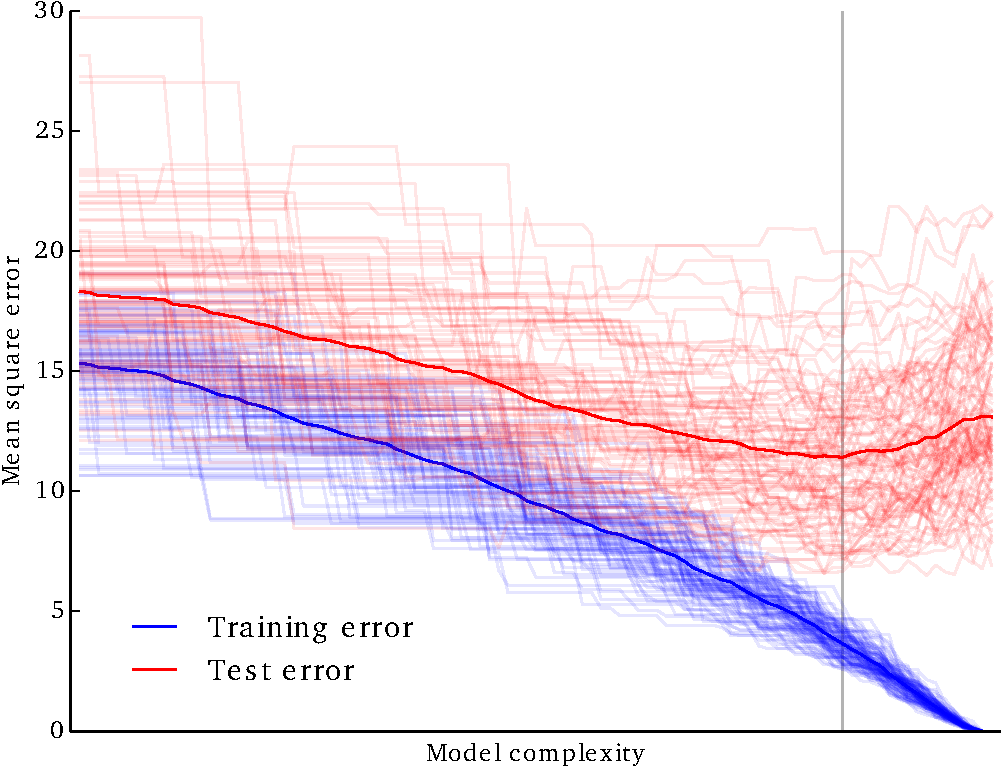
\includegraphics[width=.5\textwidth]{figures/chapter02/ch2_train_test_error.pdf}
  \caption{This plot is taken from \citet{louppe2014understanding}.
  The light blue curves show the training error while the
  light red curves show the estimated test error for 100
  pairs of training and test sets drawn at random
  from a known distribution. The thick blue curve is the average
  training error while the thick red curve is the average test error.
  It shows the necessary trade-off between the model's complexity and generalisation performance. As the model gets too complex, it starts overfitting the training data, decreasing test performance.}
  \label{fig:ch02:learning_curves}
\end{figure}
The attentive reader will notice that machine learning (ML) was only mentioned once until now, when discussing the Bayesian and frequentist interpretations of probability.
This may sound surprising as this thesis aims to build bridges between ML algorithms and the classical modelling approach. We did this on purpose as the distinction between classical modelling (as performed by domain experts, e.g. in science or engineering) and ML is often irrelevant.

We have described probabilistic modelling in generic terms that are valid for both approaches. Whether the class of models is small, made of well-understood pieces, or a deep neural network does not matter when describing the key steps to building and using a model. Even a model designed with domain knowledge usually has degrees of freedom to adapt the model to contexts. At the same time, we must not forget that learning relies on assumptions even when using deep learning with large datasets.

% The Bayesian prospect allows drawing many connections between classical modelling and ML. For example, the Bayesian interpretation of the inductive bias of a machine learning algorithm can explain its generalisation property.
Classical modelling and machine learning aim to find a model that generalises well.
On the one hand, classical modelling generally considers simple classes of models which naturally aligns with Occam's razor. It often leads to faithful models when the studied process is well understood. On the other hand, machine learning tackles problems for which classical modelling would fail because the studied phenomenon is less well understood. It does not mean ML's job is to learn a complex model of the phenomenon, quite the opposite. As depicted in \Cref{fig:ch02:learning_curves}, an ML model achieves its best predictive performance by balancing the model's complexity and goodness of fit. This behaviour is arguably observed with all ML algorithms, although defining the model's complexity is not always straightforward. A standard method to control the complexity of an ML model is to split the data into training, validation and test sets. We use the validation set to find the hyperparameters of the learning algorithm that lead to a trained model that generalises well, that is, a model that has a good balance between faithfulness (good predictive accuracy for the task of interest) and complexity. We then use these hyperparameters to learn a new model with both train and validation sets and the test set to assess how well the model generalises~\citep{hastie2009elements}.

Machine learning algorithms are sometimes described in deterministic terms. For example, a classical ML task is to predict a real value $y$ provided a set of features $\bm x$. At first glance, we might have trouble interpreting this in the probabilistic framework, limiting the scope of our previous discussion to a subset of ML algorithms. However, we can always map a deterministic model into the probabilistic framework. Indeed, deterministic learning objectives correspond to the MAP or the MLE of a probabilistic model that assumes the uncertainty a priori. For example, fitting a regression model $f_{\bm {\theta}}: \mathcal{X} \rightarrow \mathcal{Y}$ with mean squared error would lead to the same model as learning a probabilistic model via the MLE and considering a family of models that are Gaussian distributions with a fixed variance and a mean parameterised by $f_{\bm {\theta}}$. Similarly, mean absolute error corresponds to assuming a Laplace distribution. The duality between the deterministic and the probabilistic interpretations goes further if we observe that regularisation strategies correspond to the prior in the MAP, e.g. ridge regression assumes a Normal prior on the coefficients of the linear model. \citet{khan2021bayesian} discuss formally the relationships between a wide range of machine-learning algorithms and the Bayesian learning framework.

Another important aspect of modelling is to select the appropriate class of models. This choice varies with the end application which may require performing distinct types of queries on the model. In addition, the learning scenario may also differ and impacts the suitability of different models. As we will see soon, different models may lead to different inference algorithms. Some models represent the distribution of interest as a sampling procedure, while others provide access to the probability distribution. If our goal is to generate samples, we might prefer the former models, although we could also use Markov chain Monte Carlo to draw samples from the others. The following sections shed light on popular classes of probabilistic models that exhibit different advantages and shortcomings.

\section{Conclusion}
\textcolor{red}{Improve}
We have discussed the general principles of probabilistic modelling but have avoided practical technicalities. The following chapters present concrete classes of probabilistic models and the corresponding algorithms for learning and inference. In particular, \Cref{ch:02B} discusses \textbf{probablistic graphical models}~\citep[][PGMs]{koller_probabilistic_2009} and \Cref{ch:02C} reviews various \textbf{deep probabilistic models}~\citep[][DPMs]{tomczakdeep}. As its name says, the former class aims for a graphical representation of the distribution. It allows understanding the modelling assumptions, such as independence hypotheses, quickly. The latter focuses on models whose internal representations use deep neural networks. Some of these models are especially well suited for sampling and are often called \textbf{deep generative models} in this case. We discuss the particularities of each class of models and provide a thorough description of the main algorithms that perform the different queries aforementioned.

In this manuscript, we argue on multiple occasions that we shall not make a rigid distinction between graphical and deep generative models as they are just different representations of the same mathematical object. It is why we have first started our discussion with a generic introduction to probabilistic modelling that is valid for all classes of models. Some deep probabilistic models directly correspond to a graphical model, enabling abstract reasoning independent of the neural network architectures. However, for clarity, we will first introduce probabilistic graphical models. We then borrow the newly introduced notations and concepts to describe several deep probabilistic models.
